\subsection{$\PH \to \PW\PW \to \ell\nu\ell\nu$}

In this channel, the Higgs boson decays to two $\PW$ bosons, both of which decay leptonically, resulting in a signature with two isolated, oppositely charged, high-$\pt$ leptons (electrons or muons) and large $\MET$ due to the undetected neutrinos.
The analysis is very similar to that reported in~\cite{CMSobservation125}, but additionally uses an accurate lineshape model, and uses an MVA shape analysis~\cite{Chatrchyan:2012ty} for data taken at $\sqrt{s}=8\TeV$.
%Two 
%oppositely charged lepton candidates are required, 
Candidate events must contain two reconstructed leptons, with $\pt>20\GeV$ for the leading lepton, and $\pt>10\GeV$ for the
second lepton. Only electrons (muons) with $|\eta|<$2.5 (2.4) are considered in the channel.

%% ED: should the opposite-sign requirement be mentioned? It is not stated in the trigger requirements section

Events are classified into three mutually-exclusive categories, according to the number of reconstructed jets
with $\Et>30\GeV$ and $|\eta|<$4.7. The categories are characterized by different signal yields and signal-to-background ratios. In the following these are referred to as 0-jet, 1-jet and 2-jet samples. Events with more than two jets are not considered. Signal candidates are further divided into same-flavor leptons ($\Pep$, $\Pem$, $\mumu$) and different-flavor leptons ($\Elpm\Mmp$) categories. The bulk of the signal arises through direct $\PW$ decays to electrons or muons, with the 
small contribution from decays of intermediate $\tau$ implicitly included. The different-flavor lepton 0-jet and 1-jet categories are analysed with a multivariate technique, while all others make use of a selection criteria based on
sequential cuts.

In addition to high-$\pt$ isolated leptons and minimal jet activity, $\MET$ is expected to be present in signal events but
generally not in background. For this channel, a \textit{projected}~$\MET$ variable is employed. It is equal to the
component of $\MET$ transverse to the nearest lepton if the difference in azimuth between this lepton and the $\MET$ vector is less than $\pi/2$. If there is no lepton within $\pi/2$ of the direction of $\MET$ in azimuth, $\MET$ is used directly.  Since the projected ~$\MET$ resolution is degraded by pileup, the minimum of two $\MET$ observables is used. The first includes all reconstructed particles in the event, while the second uses only the charged particles associated with the primary vertex. Events with projected $\MET$ above $20\GeV$ are selected for this analysis.

The various backgrounds are suppressed using techniques described in~\cite{CMSobservation125}. Top quark backgrounds are controlled with a top-tagging technique based on soft-muon and b-jet tagging~\cite{CMS-PAS-BTV-11-003}. A minimum dilepton transverse momentum ($\pt^{\ell\ell}$) of $45\GeV$ is required, in order to reduce the $\Wjets$ background. Rejection of a third lepton passing the identification and isolation requirements reduces both $\WZ$ and $\wgamma$ backgrounds,
where in the latter case the background arises due to a photon being misidentified as an electron. The background from low mass resonances is rejected by requiring a dilepton mass $\mll>12\GeV$.

The Drell--Yan process produces same-flavor lepton pairs ($\Elp\Elm$ and $\Mp\Mm$). Additional requirements are 
therefore applied for the same-flavor final state. Firstly, the resonant component of the Drell--Yan background
is rejected by requiring a dilepton mass outside a $30\GeV$ window centered on the $\cPZ$ mass. The remaining
off-peak contribution is further suppressed by requiring the minimum of the two projected $\MET$ variables to
be greater than $45\GeV$. For events with two jets, the dominant source of fake \MET is the mismeasurement of
the hadronic recoil, and optimal performance is obtained simply by requiring $\MET>45\GeV$. Finally, the momenta of the dilepton system and of the most energetic jet must not be back-to-back in the transverse plane. These selections
reduce the Drell--Yan background by three orders of magnitude, while rejecting less than 50\% of the signal.

These requirements comprise a set of 'preselection' criteria. The preselected sample is dominated by non-resonant $\WW$ events. Figure~\ref{fig:hww2l2n_bdt_500}(a) shows the $m_{\ell\ell}$ distribution for the 0-jet different-flavor leptons category after the preselection. After preselection, a multivariate technique is employed for the different-flavor final state in the 0-jet
and 1-jet categories. In this approach, a boosted decision tree (BDT) is trained~\cite{tmva} for each Higgs boson mass hypothesis and jet category to discriminate signal from background. To enhance the signal-to-background ratio, loose $\mH$-dependent requirements are applied on $\mll$ and the transverse mass, given by:
\begin{equation} 
m_\mathrm{T}^{\ell\ell,\MET} = \sqrt{2 \pt^{\ell\ell} \MET (1-\cos\delphimetll)}\ ,
\nonumber
\end{equation}
where $\delphimetll$ is the difference in azimuth between $\MET$ and $\pt^{\ell\ell}$.

The multivariate technique employs the variables used in the preselection, and additional observables including
$\Delta R_{\Lep\Lep}$ between the leptons and the $m_\mathrm{T}^{\ell,\MET}$. For the 1-jet category the $\delphimetll$ and
azimuthal angle between the $\pt^{\ell\ell}$ and the highest $\pt$ jet are also used. The BDT-classifier distributions for $\mH=500\GeV$ are shown in Figure~\ref{fig:hww2l2n_bdt_500}(b) for the 0-jet category. BDT training is performed using $\Hww$ as signal and non-resonant $\WW$ as background. The binned BDT distributions are fitted to templates for the signal and background BDT distributions.

%% ED: $m_\mathrm{T}^{\ell,\MET}$ is a pretty nasty symbol - clarify somehow?

The 2-jet category is optimized for the VBF production mode \cite{Ciccolini:2007jr,Ciccolini:2007ec,Arnold:2008rz,Cahn:1987}, for which the cross section is roughly ten times smaller than for the gluon-gluon fusion mode. Selection criteria based on sequential sets of cuts are employed for this category.
The main requirements for selecting the VBF-type events are on the mass of the dijet system, $m_{\rm{jj}} > 450\GeV$, and on the angular separation of the two jets $\Delta \eta_{\rm{jj}} > 3.5$. An $\mH$-dependent requirement on the dilepton mass
is imposed, as well as other selection requirements that are independent of the Higgs boson mass hypothesis.

\begin{figure}[htbp]
\centering
%   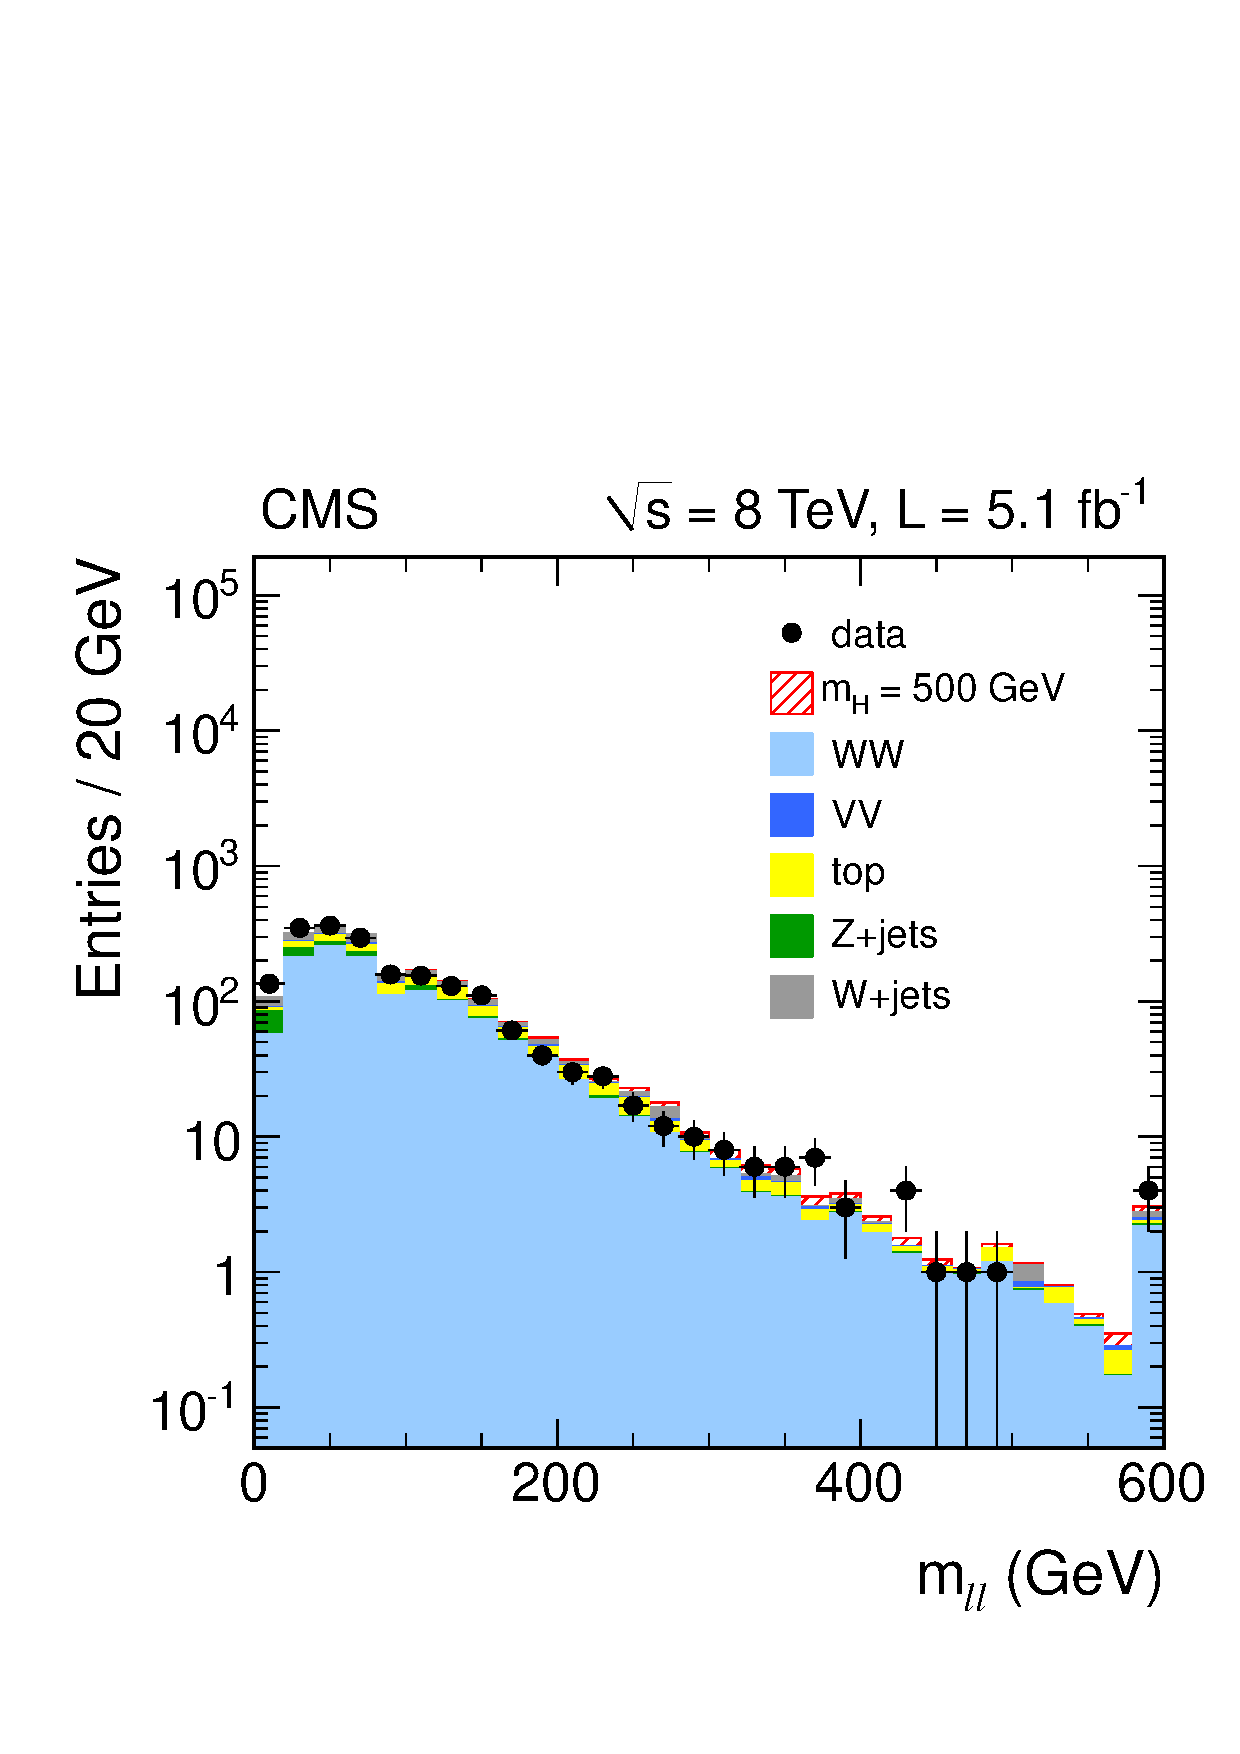
\includegraphics[width=0.49\textwidth]{plots/hww2l2n_highmass_mll500_0j.pdf}
%   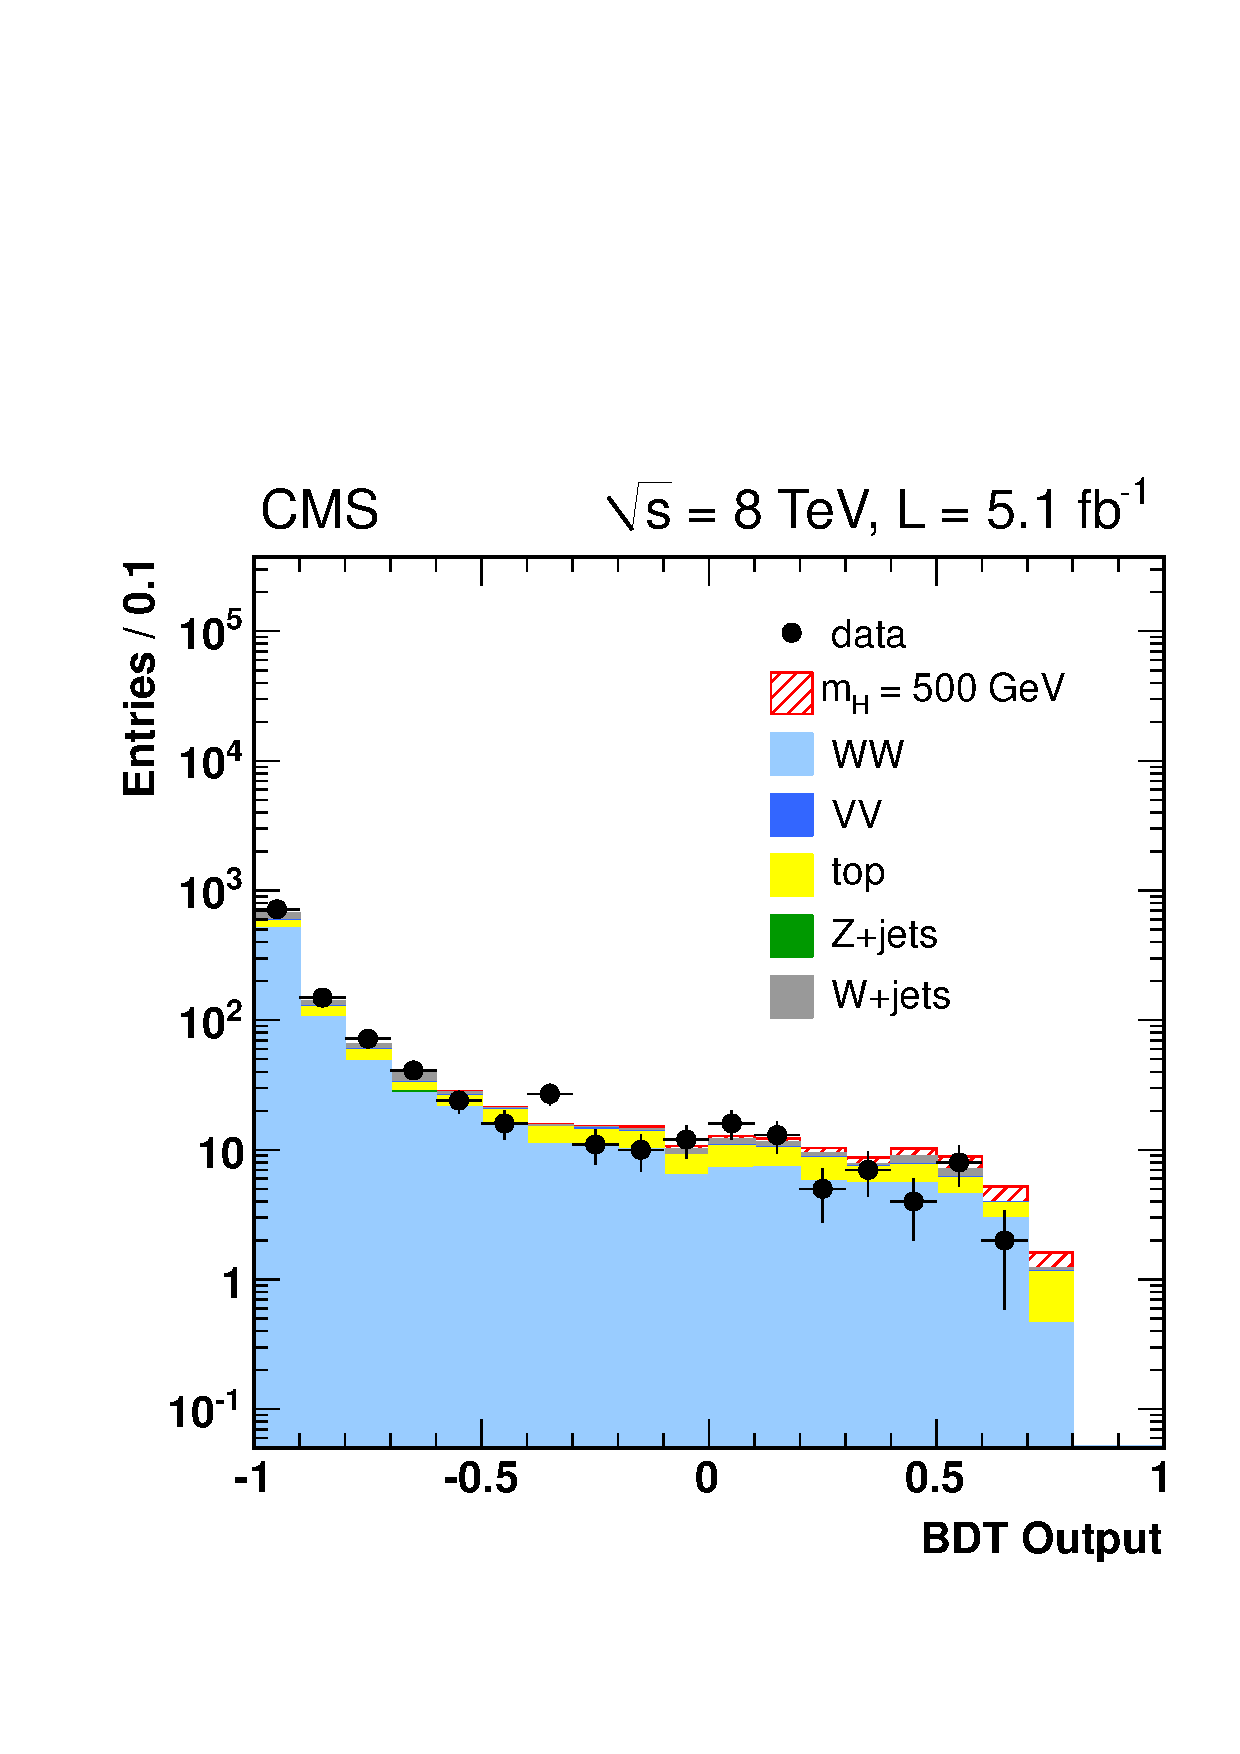
\includegraphics[width=0.49\textwidth]{plots/hww2l2n_highmass_bdt500_0j.pdf}
   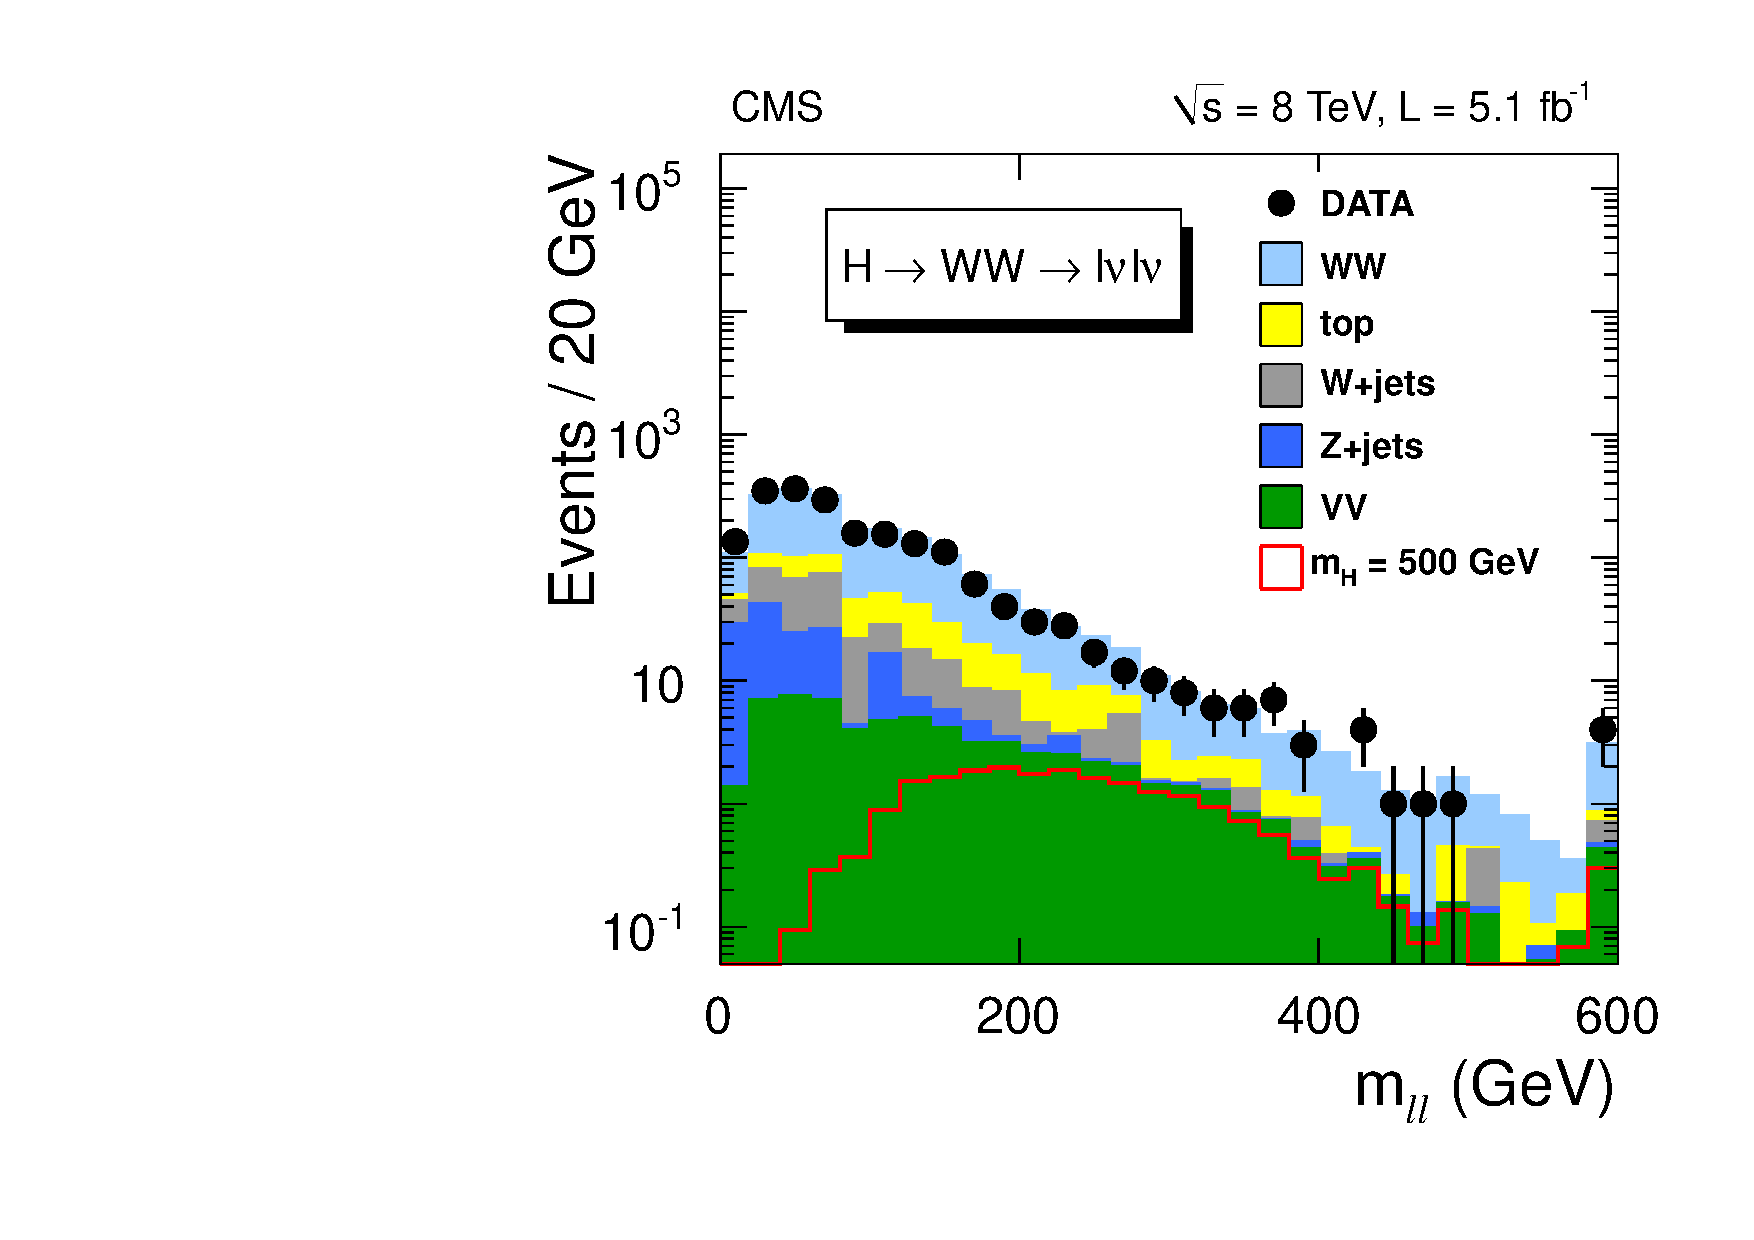
\includegraphics[width=0.49\textwidth]{figures/WW2l2nuMass.pdf}
   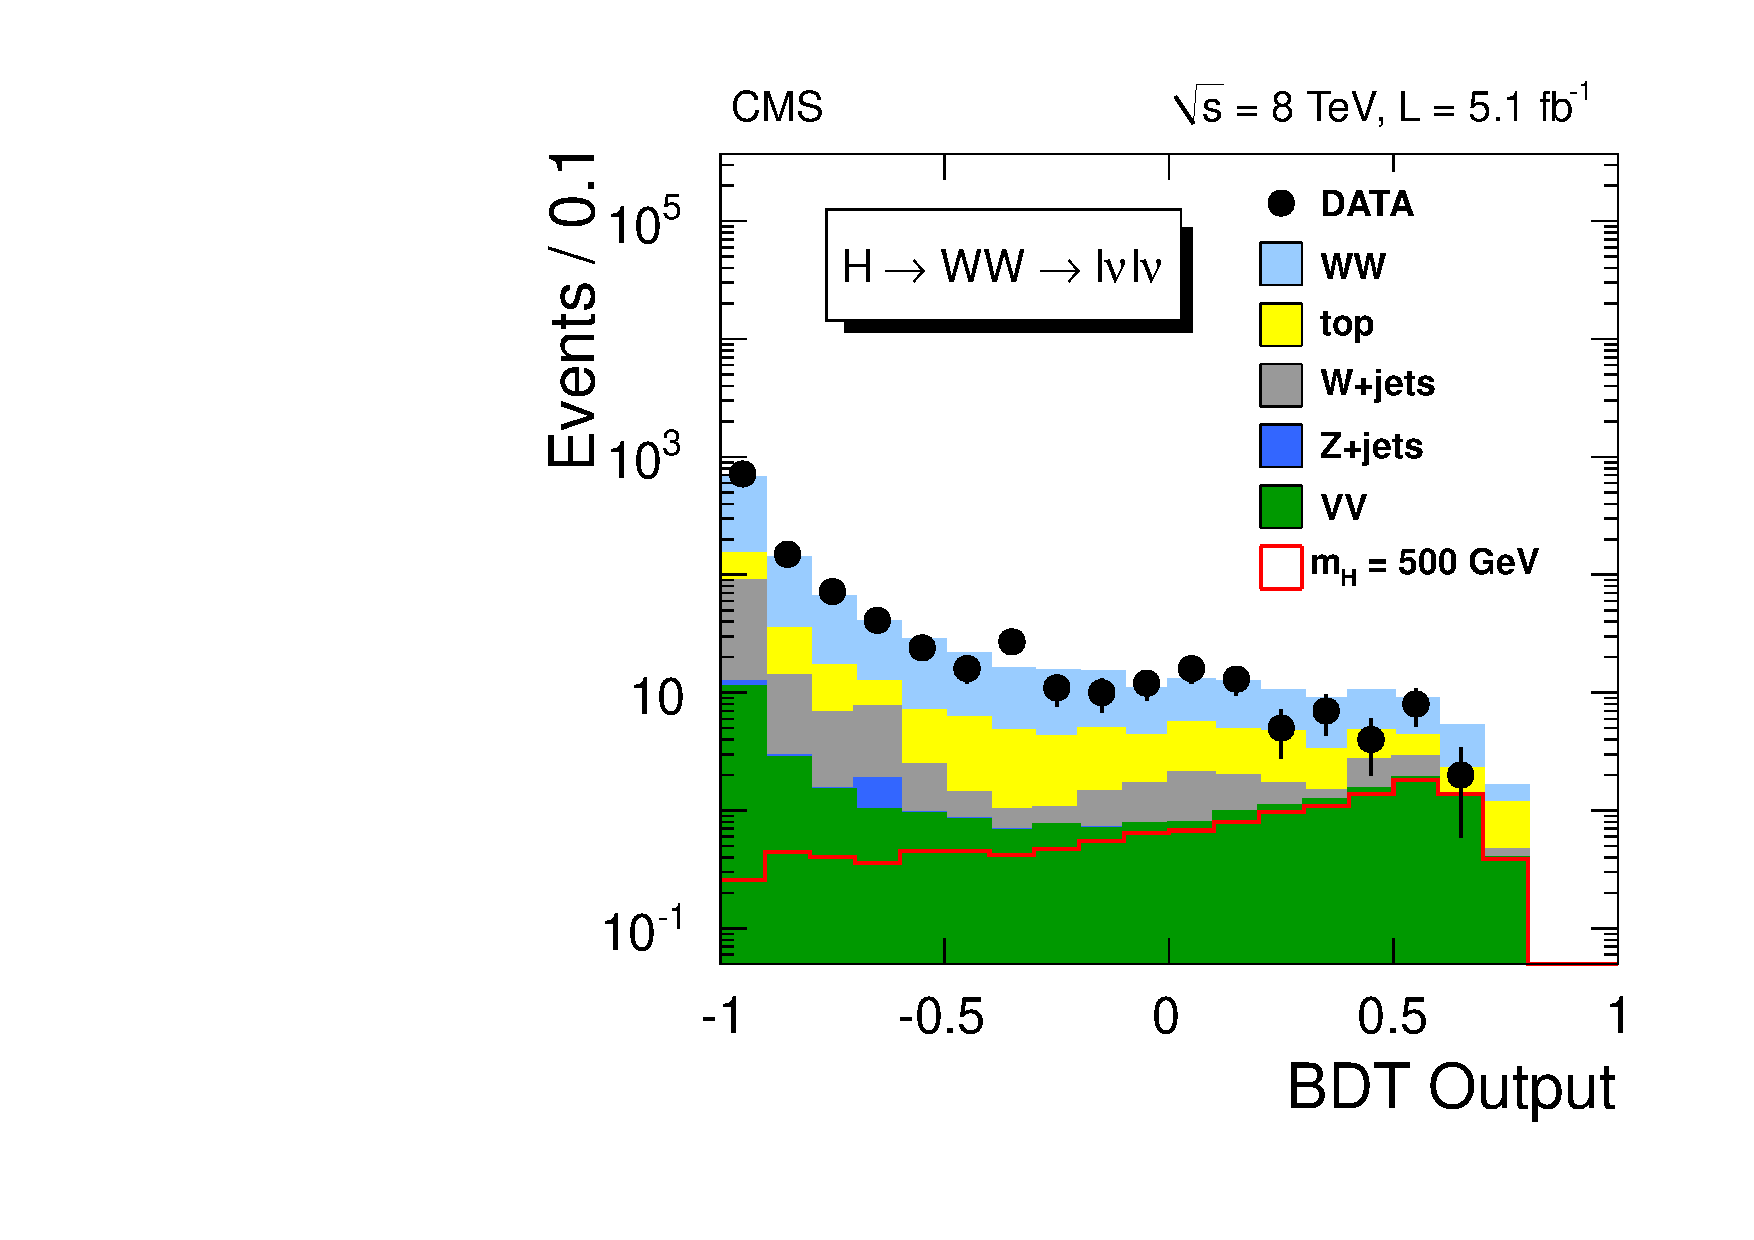
\includegraphics[width=0.49\textwidth]{figures/WW2l2nuBDT.pdf}
   \caption{ $\PW\PW \to \ell\nu\ell\nu$ channel. (a) Distributions of the dilepton mass between the
   two selected leptons in the 0-jet category, for data (points with
   error bars), for the main backgrounds (stacked histograms), and for
   a SM Higgs boson signal with $\mH= 500\GeV$ (superimposed
   histogram). The standard pre-selection is applied.  (b) BDT-classifier
   distributions for signal and background events for a SM
   Higgs boson with $\mH=500\GeV$ and for the main backgrounds at the
   BDT selection level in the 0-jet bin different-flavor final state.}
\label{fig:hww2l2n_bdt_500}
\end{figure}

The backgrounds that remain after applying the final selection criteria are estimated by a combination of techniques~\cite{CMSobservation125}. The $\ttbar$ background is estimated by extrapolation from the observed 
number of events with the b-tagging cut inverted. The Drell--Yan background measurement is based on extrapolation
from the observed number of $\Pe^+\Pe^-$, $\Pgm^+ \Pgm^-$ events with the $\cPZ$-veto cut inverted. The background 
of $\PW$+jets and QCD multi-jet events is estimated by measuring the number of events with one lepton passing a loose
cut on isolation. The probability for such loosely-isolated fake leptons to pass the tight isolation cut is measured in
data using multi-jets events. The non-resonant $\WW$ contribution is estimated from simulation.

Experimental effects, theoretical predictions, and the choice of event generators are considered as sources of
uncertainty, and their impact on the signal efficiency is assessed. The impact on the kinematic distributions is also considered for the BDT analysis. The overall signal efficiency uncertainty is estimated to be about 20\%, and is
dominated by the theoretical uncertainty associated with missing QCD higher-order corrections and PDF uncertainties. The total uncertainty on the background estimation in the $\Hww$ signal region is about 15\%, dominated by the
statistical uncertainty on the observed number of events in the background control regions.

After applying the final selections, no evidence of a SM Higgs boson is observed over the mass range considered in this paper. Upper limits are derived on the ratio of the product of the Higgs boson production cross section and the $\Hi \to \WW$ branching fraction, $\sigma_{\Hi} \times \mathrm{BR}(\Hi \to \WW)$, to the SM expectation. The observed and expected upper limits with all categories combined are shown in Figure~\ref{fig:hwwlvlvlim}. At least part of the excess observed at
low masses may be ascribed to the presence of the new boson at mass about 125 GeV that is not accounted for in the analysis.

\begin{figure}[htbp]
  \centering
%  \subfigure[]{
%  \includegraphics[width=0.48\textwidth]{plots/hwwlvlvlimit8tev.pdf}
%  }  
%   \subfigure[]{ 
  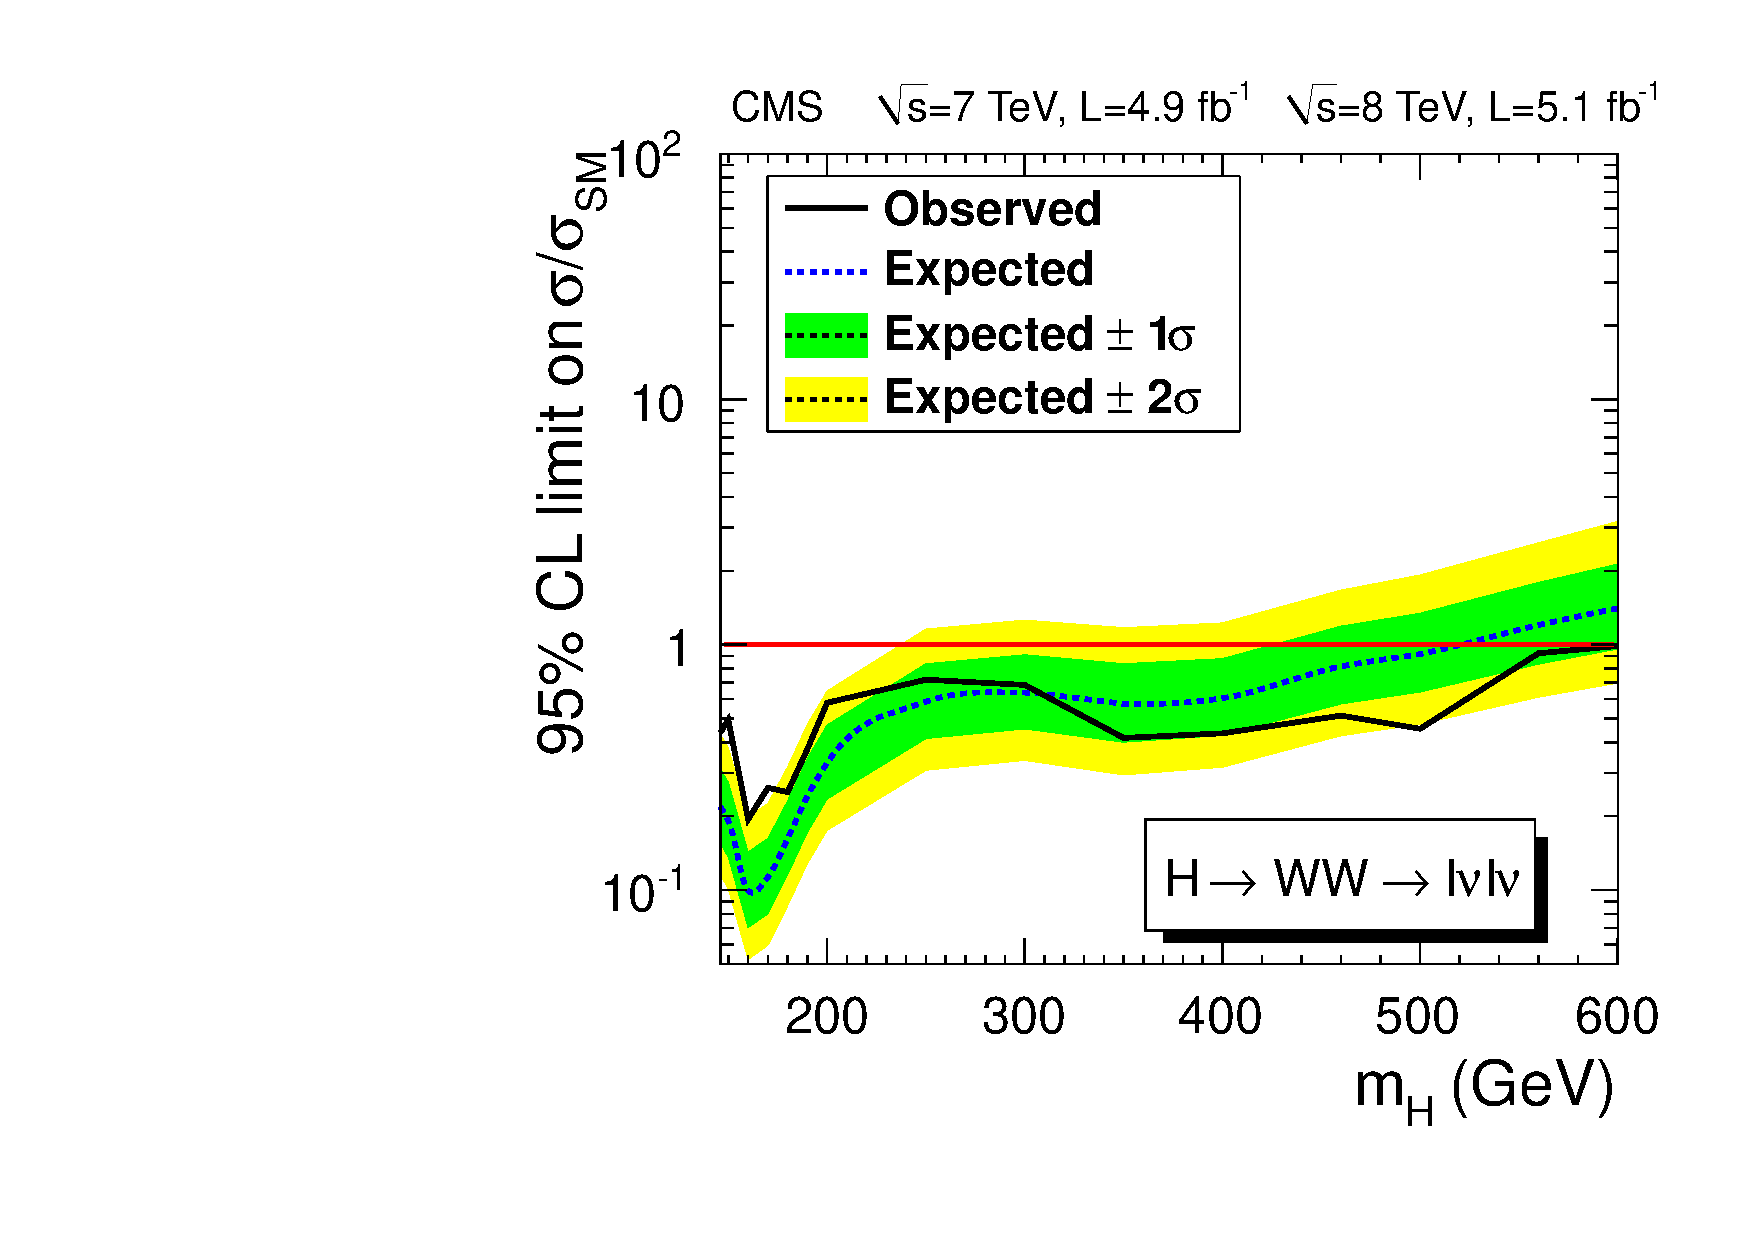
\includegraphics[width=0.6\textwidth]{figures/WW2l2nuLimit.pdf}
%  }   
  \caption{\label{fig:hwwlvlvlim}Observed (solid) and expected
    (dashed) 95\% CL upper limit on the ratio of the product of production cross
    section and branching ratio to the SM expectation for the Higgs boson obtained using
    the asymptotic CL${}_{\textrm{S}}$ technique in the $\PW\PW \to \ell\nu\ell\nu$ channel. The 68\% and 95\%
    ranges of expectation for the background-only model are also shown
    with green and yellow bands, respectively. The solid line at 1
    indicates the SM expectation.} 
%The limit combines data from both
%    7 TeV and 8 TeV collisions.},
\end{figure}

\subsection{$\PH \to \PW\PW \to \ell\nu \rm{qq}$}

The $\WW$ semileptonic channel has the largest branching fraction of all the channels presented in this paper.
Its advantage over the fully leptonic final state is that it has a reconstructable Higgs boson mass peak~\cite{intro2}. This
comes at the price of a large \PW+jets background. The level to which this background can be controlled
largely determines the sensitivity of the analysis. 

The reconstructed electrons (muons) are required to have 
$\PT>35(25)\GeV$, and are restricted to $|\eta|<2.5(2.1)$.
The jets are required to have 
$\PT>30\GeV$ and $|\eta|<2.4$, and to not
overlap with the leptons, 
with the overlap determined by a cone around the lepton axis of radius $\Delta R = 0.3$. 
%The analysis is performed in four categories. Events with electrons and muons,
%and also with two or three jets located within the tracker acceptance ($|\eta| < 2.4$) and with
%$\PT>30\GeV$ are analysed separately.
%Jets that overlap isolated leptons are not considered, with the overlap
%determined by a cone around the lepton axis of radius $\Delta R = 0.3$. Since initial and final
%state gluon radiation can result in an extra jet, only events with exactly two or three jets
%are selected for the analysis.
Events with the electrons and muons, and with exactly two or three jets are analysed separately,
giving four categories in total.
%Events with electrons and muons are analysed separately. Since initial and final state gluon radiation can result in an additional jet, events with two or three jets above are selected for the analysis, and also analysed separaetly,
%giving four analysis categories in total. Jets are required to have $|\eta|<2.4$ and $\PT>30\GeV$, and jets that overlap isolated leptons are not considered, with the overlap determined by a cone around the lepton axis of radius $\Delta R = 0.3$. 
%% ED: Do we really mean *isolated* lepton here? 
The combination of the two highest-$\PT$ jets is assumed as the hadronic $\PW$ candidate. According to simulation, in the case of 2(3)-jet events, the correct jet-combination rate varies from 68(26)\% for $\mH = 200\GeV$ to 88(84)\% for
$\mH = 600\GeV$. Events with an incorrect dijet combination result in a broad non-peaking background in the $m_{\WW}$ spectrum.

The leptonic $\PW$ candidate is reconstructed from the $(\ell,\MET)$ system. Events are required to have $\MET>\text{30(25)}\GeV$ for the electron(muon) categories. To reduce the background from processes that do not
contain $\PW\to\ell\nu$ decays, requirements of $m_{\rm{T}}^{\ell,\MET}>30\GeV$ and
$|\Delta\phi_{\textrm{leading jet,\MET}}| >$ 0.8 (0.4) are imposed for electrons (muons). These criteria reduce the QCD multi-jet background, for which in many cases the $\MET$ is generated by the overestimate of the energy of a jet.

To improve the $m_{\WW}$ resolution, both $\PW$ candidates are constrained in a kinematic fit to the $\PW$-boson
mass to within its known width, with the longitudinal component of the neutrino momentum, $|p_{\textnormal{z}}|$ unknown. The ambiguity in the second-order kinematic equation is resolved by taking the solution that yields the smaller $|p_{\textnormal{z}}|$ value for the neutrino.  

%% ED: What does 'constrained to the W mass to within its known width' mean? Is it just constrained to the W mass, or allowed to float within some range?

To exploit the differences in kinematics between signal and background events, a likelihood discriminant is constructed
that incorporates a set of variables that best distinguishes the Higgs signal from the \PW+jets background. 
These variables comprise five angles between the Higgs decay products, that fully describe the Higgs production kinematics~\cite{Gao:2010qx}; the $\PT$ and rapidity of the $\WW$ system; and the lepton charge.
The likelihood discriminant is optimized with dedicated simulation samples for several discrete Higgs boson mass hypotheses,
for each lepton flavor ($\Pe$, $\Pgm$) and for each jet multiplicity (2-jet, 3-jet) independently. Four different optimizations are therefore obtained per mass hypothesis. For each of them, events are retained if they
survive a simple selection on the likelihood discriminant, chosen in order to optimise the expected limit for the Higgs cross-section.

%% ED: Please check that I have reworded the last sentence correctly, and preserved the meaning.

To extract simultaneously the relative normalizations of all background components in the signal region, an
unbinned maximum likelihood fit is performed on the invariant mass distribution of the dijet system, $m_{jj}$.
The fit is performed independently for each Higgs boson mass hypothesis. The signal region corresponding to the $\PW$
mass window, $65\GeV < m_{jj} < 95\GeV$, is excluded from the fit. The shape of the $m_{jj}$ distribution for the
$\PW$+jets background is taken from simulation for Higgs boson mass hypotheses at or below $200\GeV$. For higher masses,
insufficient numbers of simulated events are available, and the shape is therefore described analytically using an exponential function. The overall normalization of the \PW+jets component is allowed to vary in the fit. The shapes for
other backgrounds (electroweak diboson, \ttbar, single top, and Drell--Yan plus jets) are based on simulation, and their
normalizations are constrained to theoretical predictions, within the corresponding uncertainties.
The multijet background normalization is estimated from data by relaxing lepton isolation and identification requirements.
Its contribution to the total number of events is evaluated from a separate two-component likelihood fit to the $m_{\rm{T}}^{\ell,\MET}$ distribution, and constrained in the $m_{jj}$ fit according to this fraction within
uncertainties. For electrons, the multijet fraction accounts for several percent of the event sample, depending on the
number of jets in the event, while for muons it is negligible.


Limits are established based on the measured invariant mass of the $\WW$ system, $m_{\ell\nu jj}$. The
binned shapes of
$m_{\ell\nu jj}$ for total background, signal and data for each mass hypothesis and event category are
constructed as
input to the limit-setting procedure. The $m_{\ell\nu jj}$ shape for the major background, \PW+jets,
is extracted from data as a linear combination of the shapes measured in two signal-free sideband
regions of $m_{jj}$ ($55\GeV <m_{jj} < 65\GeV$,
$95\GeV < m_{jj} < 115\GeV$). The relative fraction of the two sidebands is motivated through
simulation, separately for
each Higgs boson mass hypothesis, by minimizing the $\chi^2$ between the interpolated shape in the
signal region and the expected one. The $m_{\ell\nu jj}$ shape for multijet background events is
obtained from data with the procedure described above.
All other background categories use the $m_{\ell\nu{}jj}$ shape
from simulation.

The $m_{jj}$ and $m_{\ell\nu jj}$ distributions with final background estimates are 
shown in Figure~\ref{fig:lvjjfits}, with
selections optimized
for a $500\GeV$ Higgs boson mass hypothesis, for the $(\Pgm,2\rm{jets})$ category. 
The final background $m_{\ell\nu{}jj}$ distribution is obtained by summing
up all the individual contributions.
To avoid statistical fluctuations due to the low event count,
the distribution is fit with an exponential function. This function
is then used for the
limit evaluation. All uncertainties arising from interpolation and fit procedures are propagated to
the limit calculation as
systematic uncertainties.


%Limits are established based on the measured invariant mass of the $\WW$ system, $m_{\ell\nu jj}$. The binned shapes of
%$m_{\ell\nu jj}$ for total background, signal and data for each mass hypothesis and event category are constructed as
%input to the limit-setting procedure. The $m_{\ell\nu jj}$ shape for the major background, \PW+jets, is extracted from data as a linear combination of the shapes measured in two signal-free sideband regions of $m_{jj}$ ($95\GeV <m_{jj} < 115\GeV$,
%$55\GeV < m_{jj} < 65\GeV$). The relative fraction of the two sidebands is motivated through simulation, separately for
%each Higgs boson mass hypothesis, by minimizing the $\chi^2$ between the interpolated shape in the signal region and the expected one. The $m_{\ell\nu jj}$ shape for multijet background events is obtained from the data sample selected for the $m_{jj}$ fit and normalized according to the fit results. All other background categories use the $m_{\ell\nu{}jj}$ shape
%from simulation.

%% DN: 'extrapolated' -> 'interpolated' I think?

%Examples of the $m_{jj}$ and $m_{\ell\nu jj}$ fits are shown in Figure~\ref{fig:lvjjfits}, with selections optimized
%for a $500\GeV$ Higgs boson mass hypothesis, for the $(\Pgm,2\rm{jets})$ category. The distributions of the interpolated 
%\PW+jets background in the signal region are also shown. Because of the low event count, the shapes are regularized by
%means of an exponential fit. The uncertainties from both fits are propagated to the limit calculation as 
%systematic uncertainties.

\begin{figure}[htbp]
  \centering
  \subfigure[]{
%  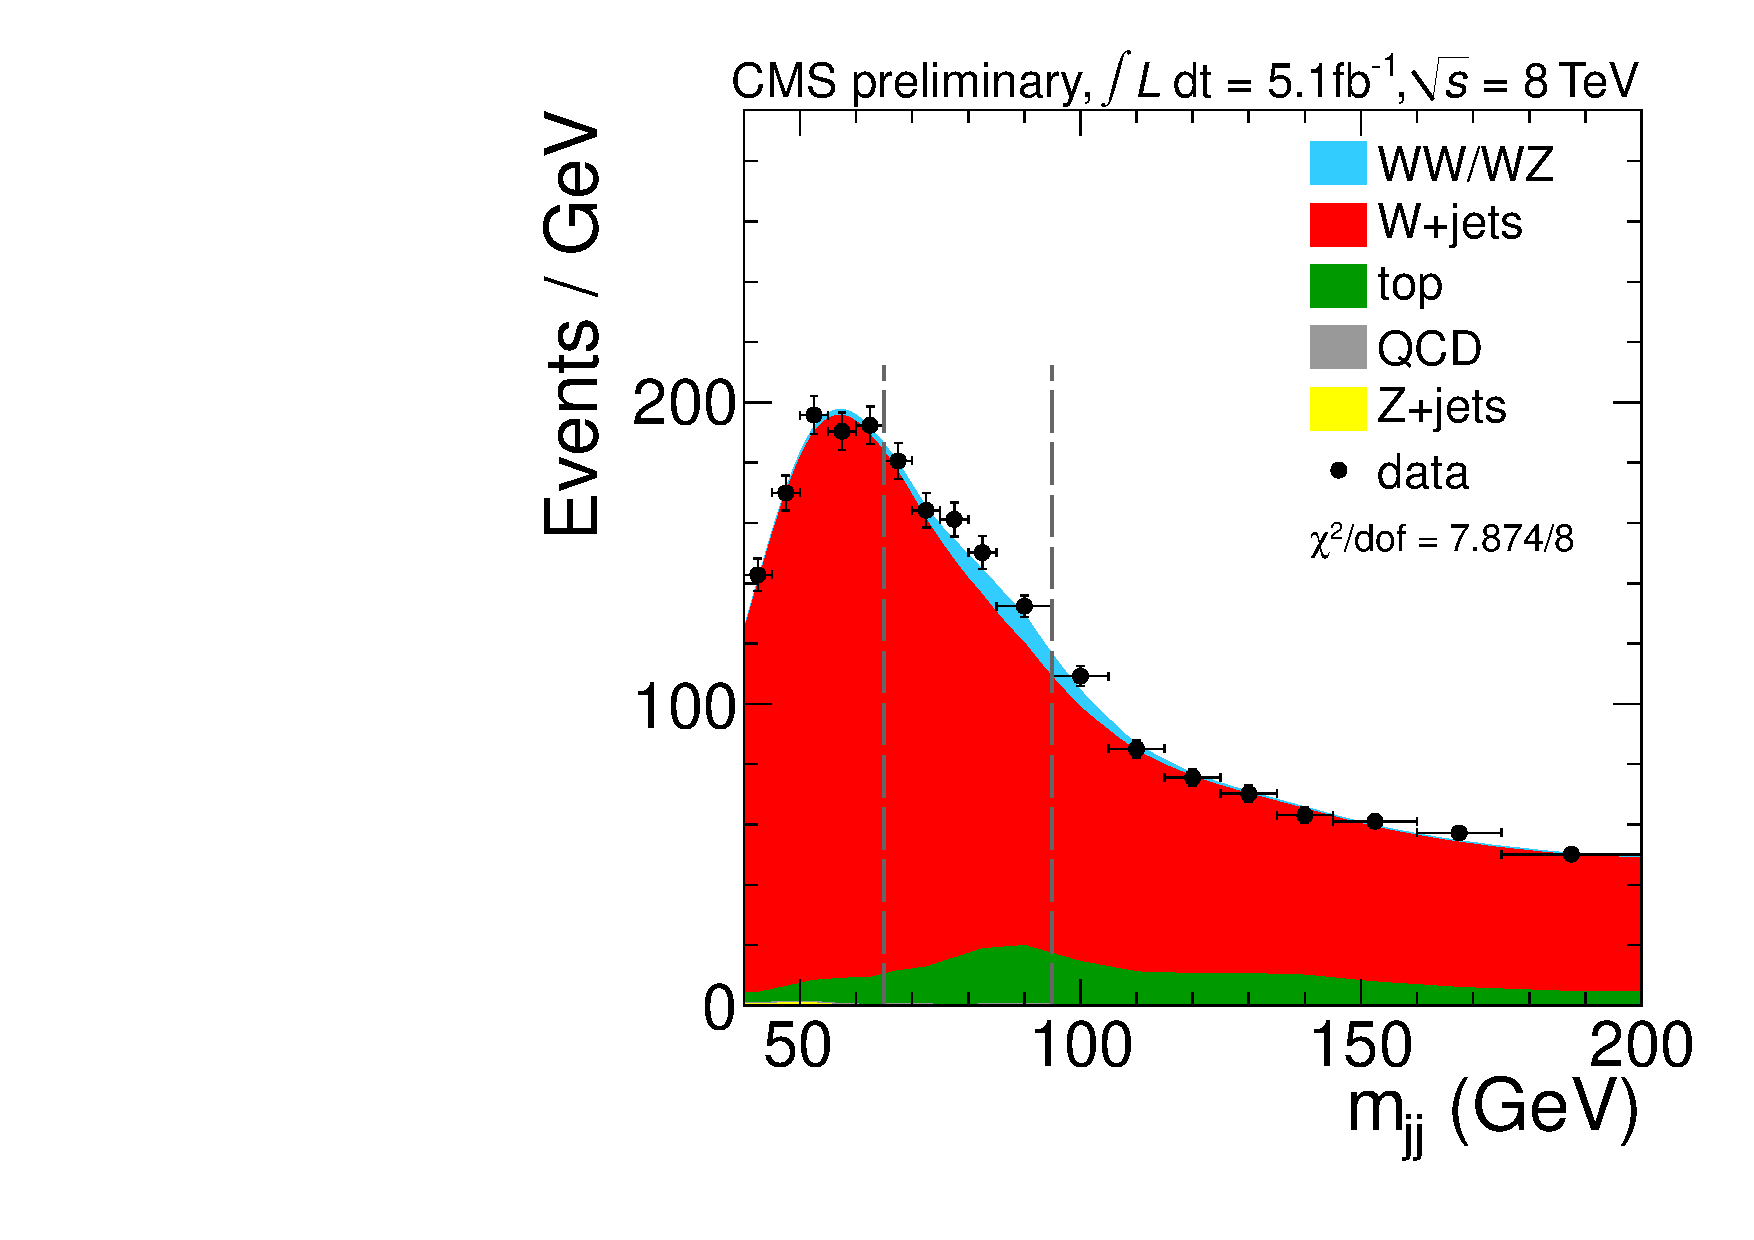
\includegraphics[width=0.48\textwidth]{plots/H500_Mjj_Muon_2jets_Stacked.pdf}
  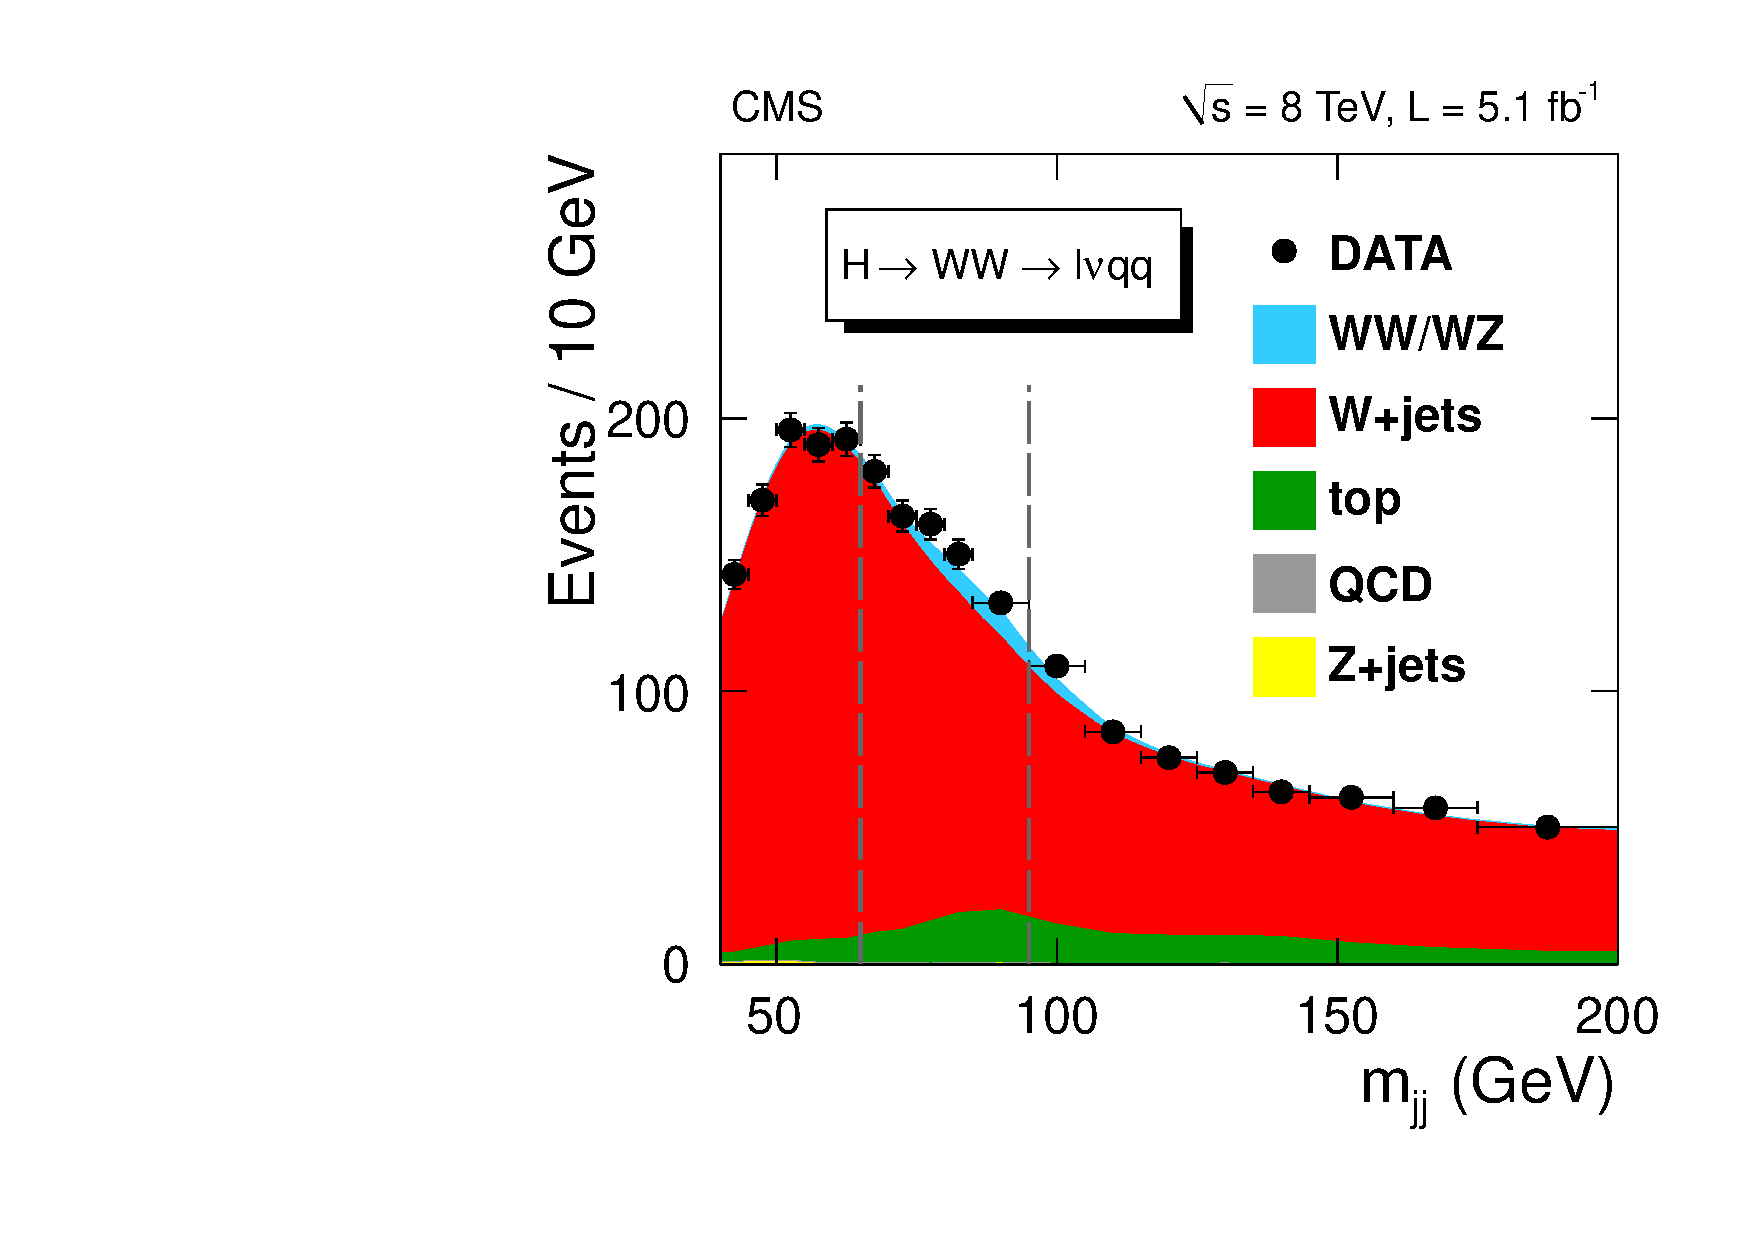
\includegraphics[width=0.48\textwidth]{figures/WW2l2qMjj.pdf}
  }  
   \subfigure[]{ 
%  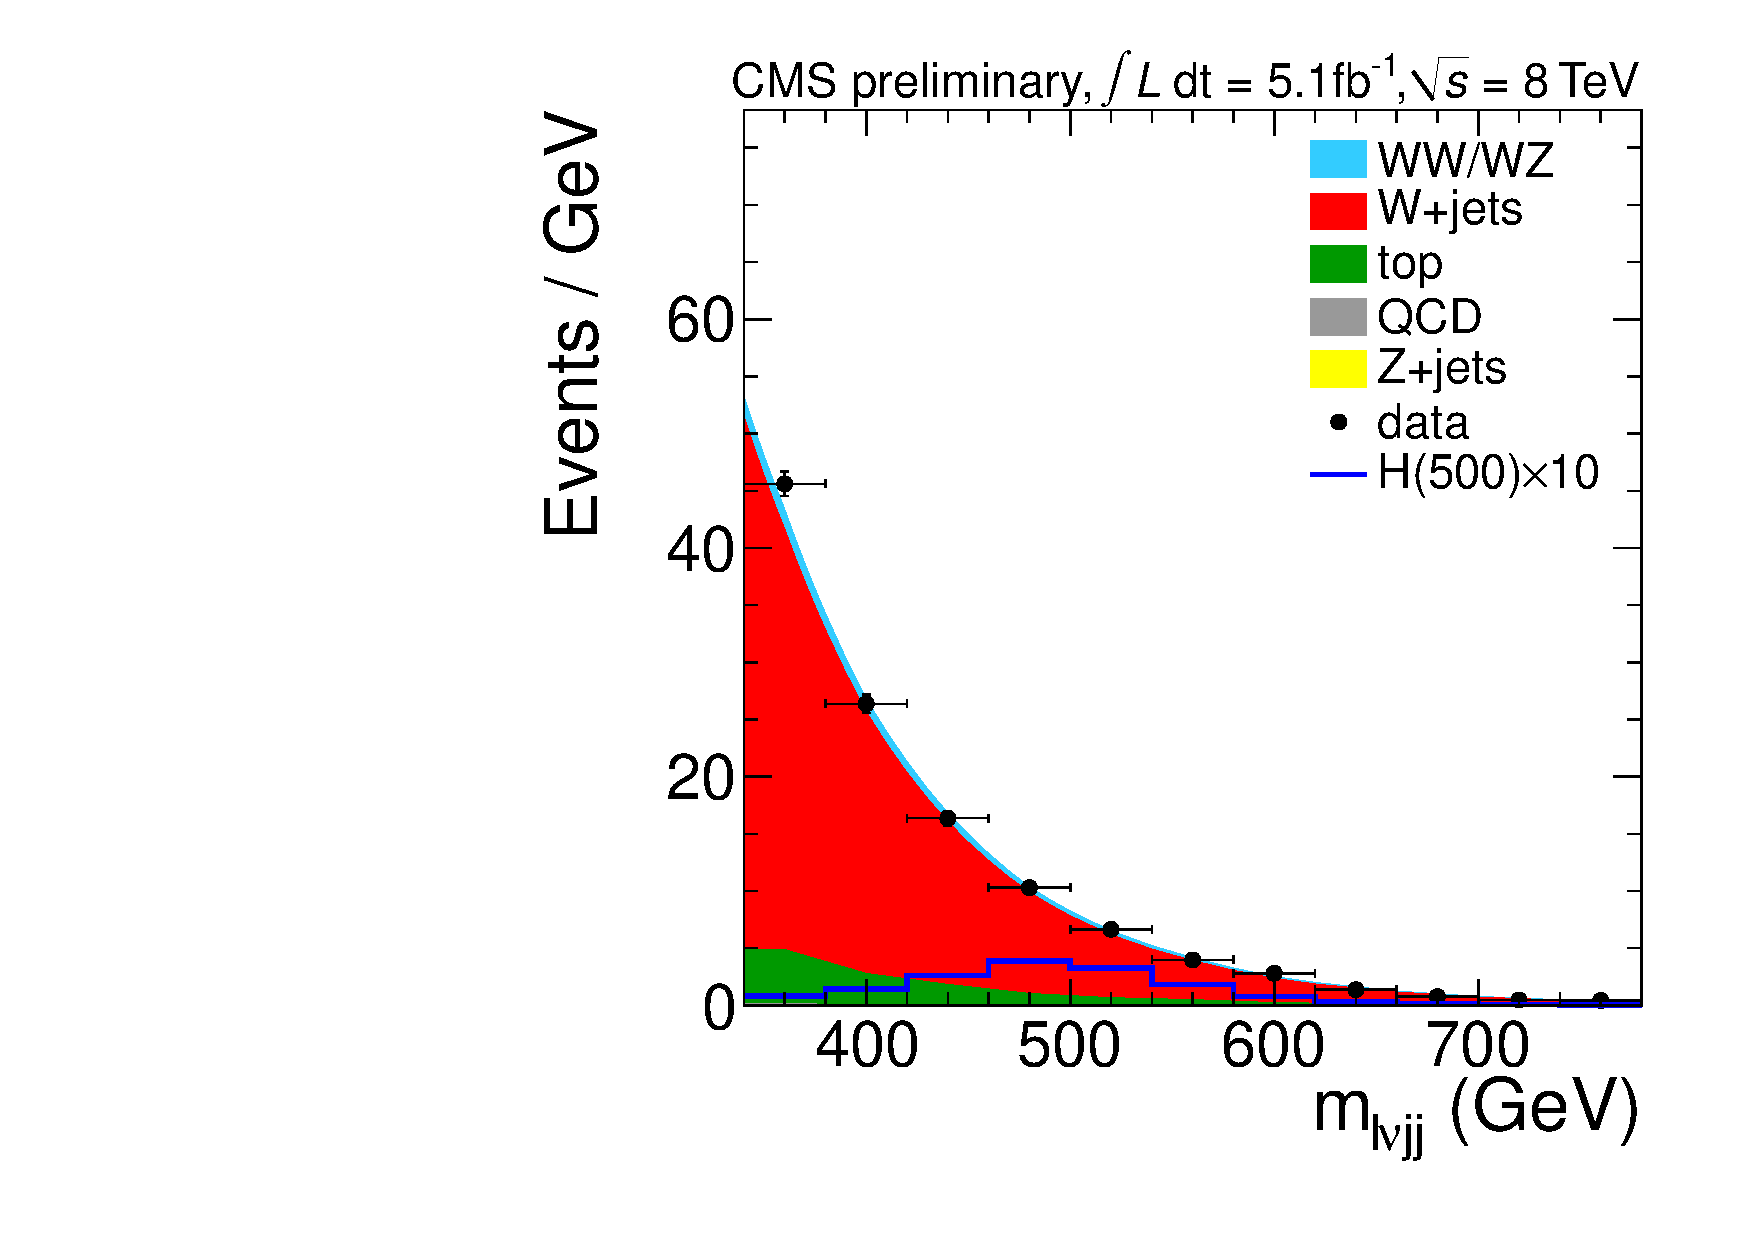
\includegraphics[width=0.48\textwidth]{plots/H500_Mlvjj_Muon_2jets_Stacked.pdf}
  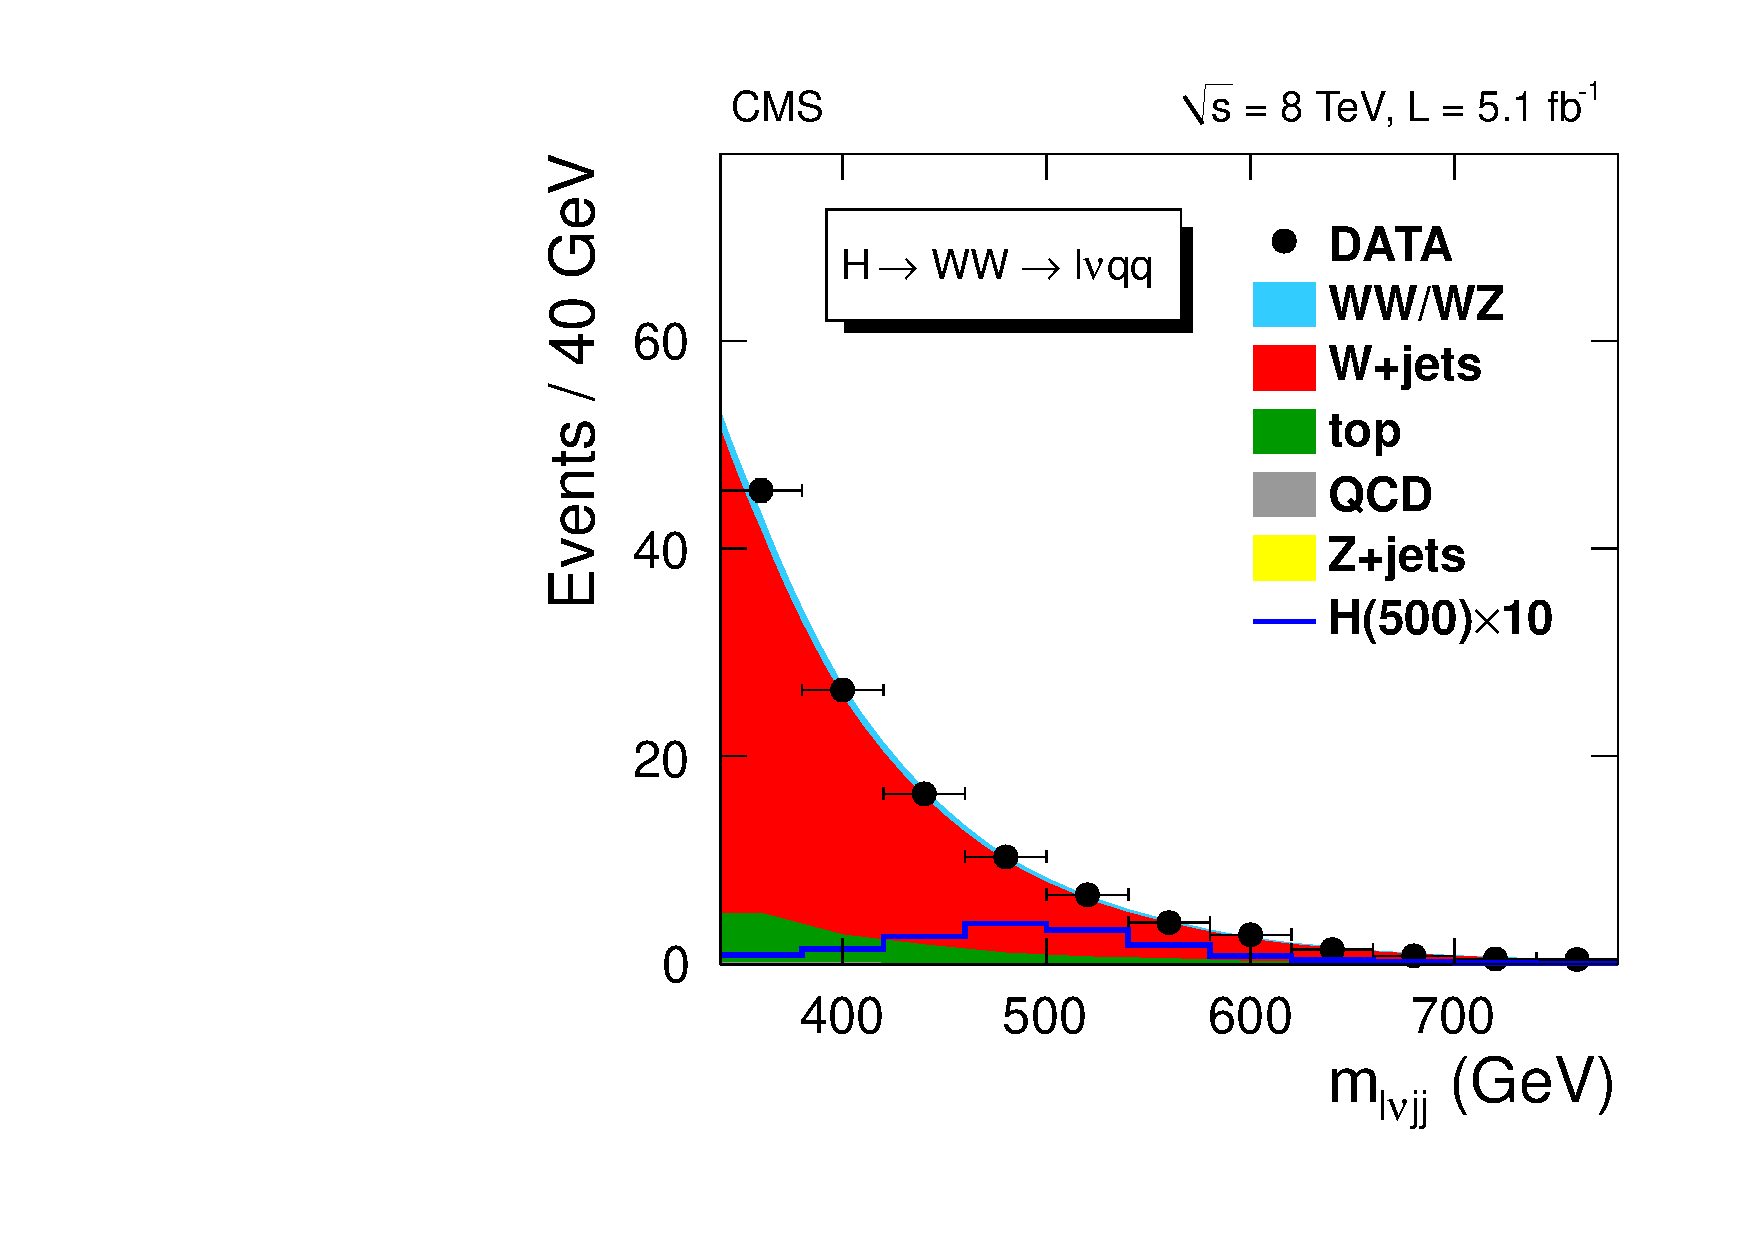
\includegraphics[width=0.48\textwidth]{figures/WW2l2qMass.pdf}
  }   
%  \subfigure[]{ 
%  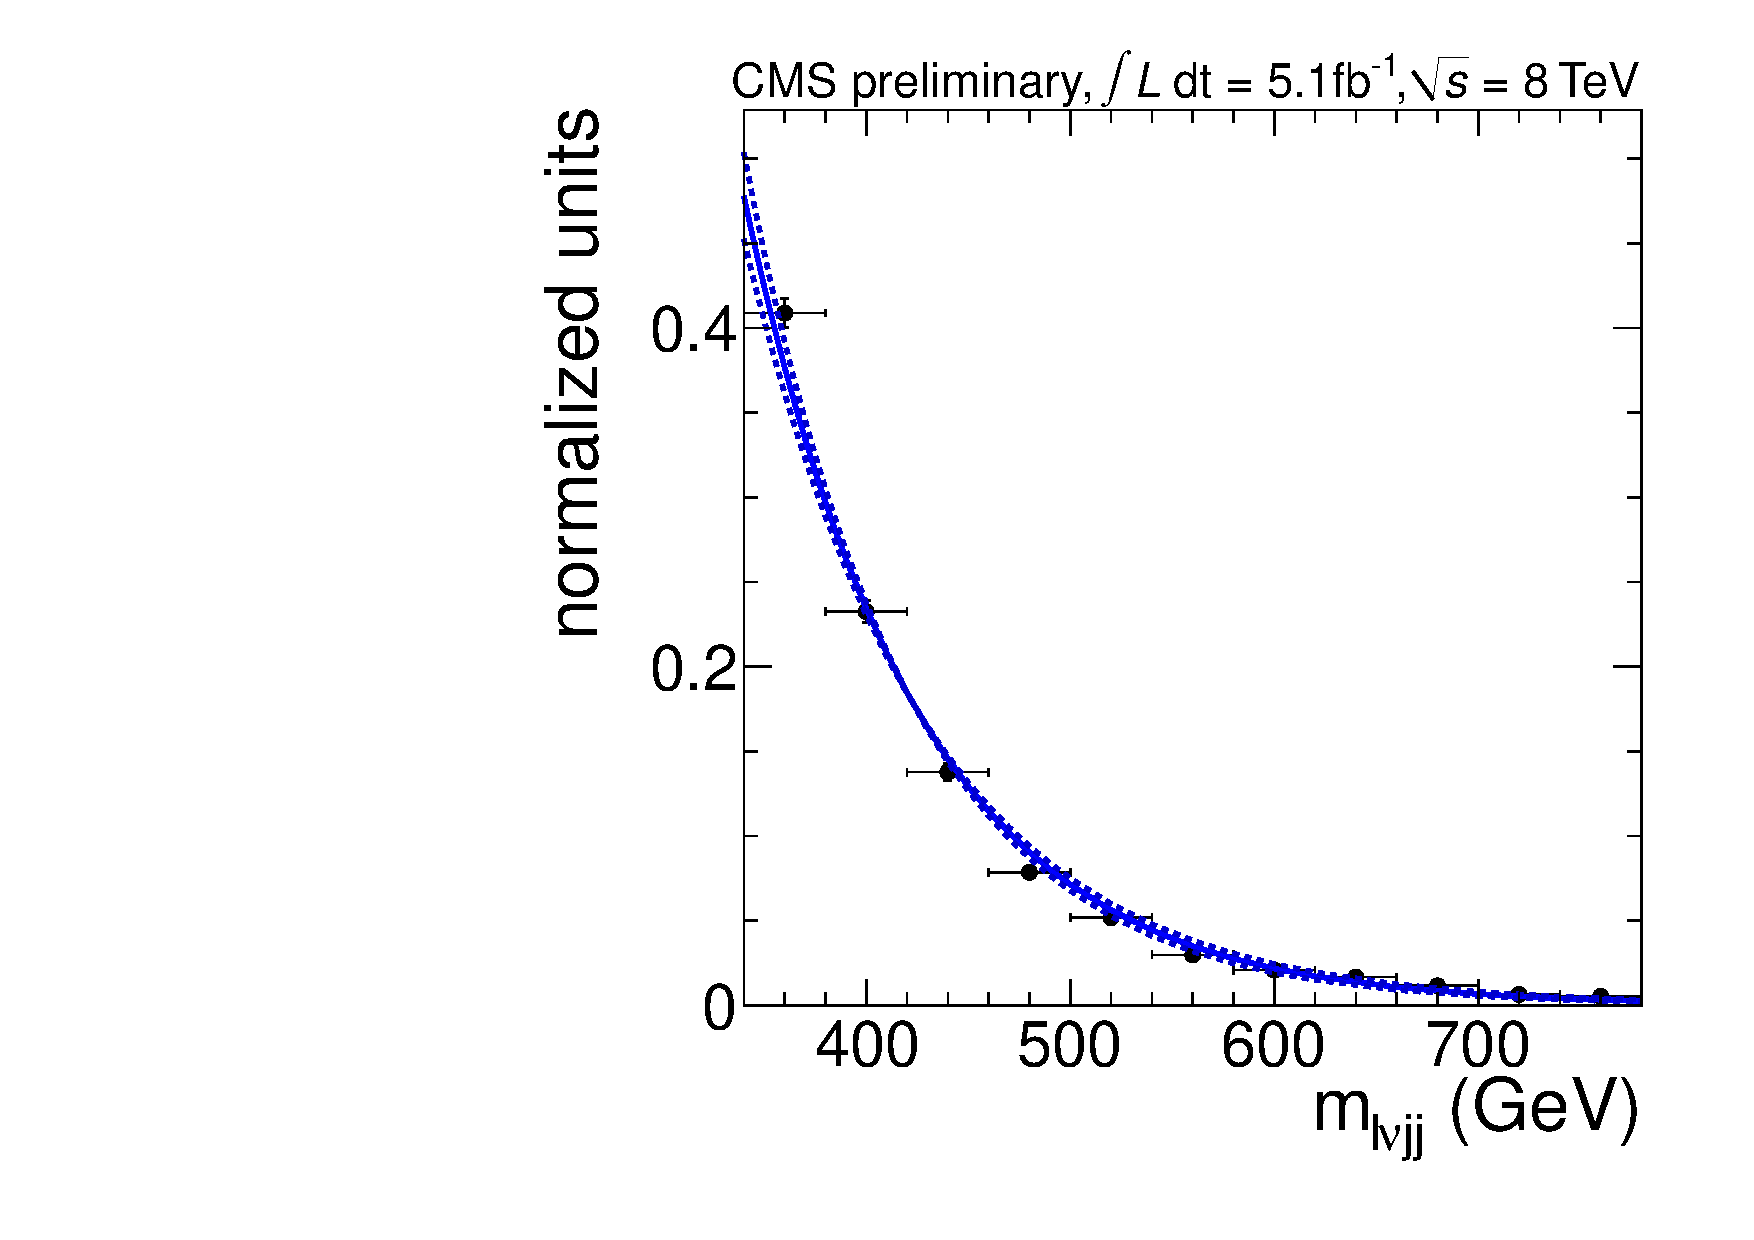
\includegraphics[width=0.32\textwidth]{plots/H500_Mlvjj_Muon_2jets_WpJShape.pdf}
%  }  
%  \caption{\label{fig:lvjjfits} Fit plots for the mass hypothesis
%    $\mH=500\GeV$, muon 2-jet category in the $\PH \to \PW\PW \to \ell\nu \rm{qq}$ channel.  (a) The dijet invariant mass
%    distribution with the fit projections of the background components.
%    The vertical lines corresponds to the signal region of this analysis
%    $65\GeV < m_{jj}
%    < 95\GeV$.  %(c) The distribution of the extrapolated background
%    (b) The $\WW$ invariant mass distribution with the fit projections of
%    the background components in the signal region.
%    The black symbols represent the data.}
%    interpolated points, while the blue curve is the smooth
%    parametrization using an exponential function.}  
%    The dashed bands
%    show the envelope of the systematic uncertainty in the shape
%    extrapolation. }
  \caption{\label{fig:lvjjfits} Invariant mass distributions for the
    $\mH=500\GeV$ mass hypothesis, $(\Pgm,2\rm{jets})$ category in the
    $\PH \to \PW\PW \to \ell\nu \rm{qq}$ channel.
    (a) The dijet invariant mass
    distribution with the major background contributions.
    The vertical lines corresponds to the signal region of this analysis
    $65\GeV < m_{jj}
    < 95\GeV$.
    (b) The $\WW$ invariant mass distribution with the major background
    contributions in the signal region.
    }
\end{figure}

The largest source of systematic uncertainty is due to $m_{\ell\nu jj}$-shape uncertainty of the \PW+jets background.
The only other uncertainty assigned to background is the normalization uncertainty from the $m_{jj}$ fit. Both of these 
uncertainties are estimated from data. All other systematic uncertainties are applied to signal processes. The dominant 
signal uncertainties include theoretical uncertainties for the cross section (14-19\% for gluon fusion)~\cite{LHCHiggsCrossSectionWorkingGroup:2011ti} and exclusive jet binning effects on scale (4-28\%), as well as the 
efficiency of the likelihood selection (10\%). The latter effect is computed by taking the relative difference in efficiency 
between data and simulation using a control sample of top pair events in data. These events are good proxies for the signal,
since in both cases the primary production mechanism is gluon-gluon fusion, and the semi-leptonic final states contain
decays of two W bosons.

The upper limits on the ratio of the production cross section for the Higgs boson compared to the SM expectation are 
presented in Figure~\ref{fig:hwwlvjjlim}. 

\begin{figure}[htbp]
  \centering
%   \subfigure[]{
%  \includegraphics[width=0.48\textwidth]{plots/hwwlvjjlimit8tev.pdf}
%   }
%  \subfigure[]{
  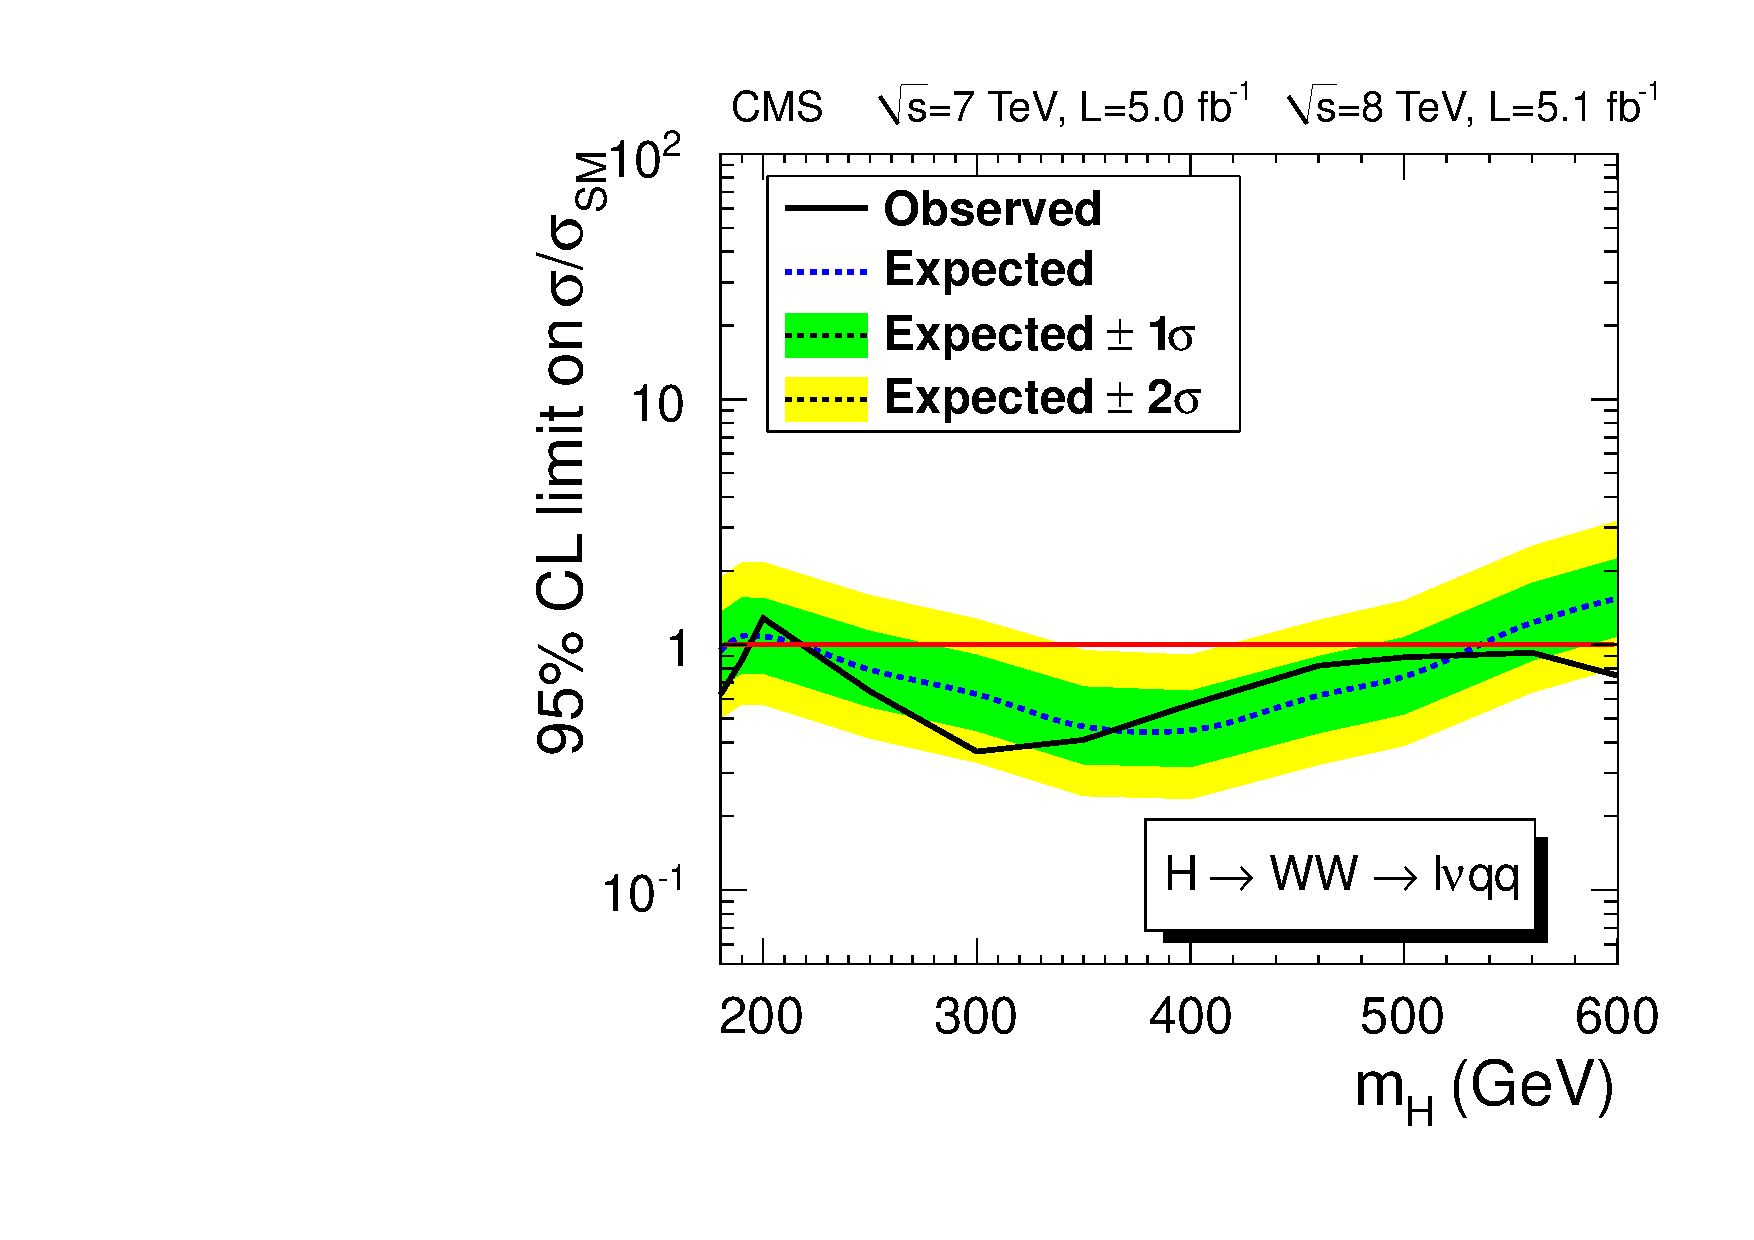
\includegraphics[width=0.6\textwidth]{figures/WW2l2qLimit.pdf}
%  }
  \caption{\label{fig:hwwlvjjlim} Observed (solid) and expected
  (dashed) 95\% CL upper limit on the ratio of the product of production cross
  section and branching ratio to the SM expectation for the Higgs boson in the WW
  semileptonic channel.}  
%The limit combines data from both 7 TeV and 8
%  TeV collisions.}
\end{figure}
